% Indicate the main file. Must go at the beginning of the file.
% !TEX root = ../main.tex

%%%%%%%%%%%%%%%%%%%%%%%%%%%%%%%%%%%%%%%%%%%%%%%%%%%%%%%%%%%%%%%%%%%%%%%%%%%%%%%%
% 02_methods
%%%%%%%%%%%%%%%%%%%%%%%%%%%%%%%%%%%%%%%%%%%%%%%%%%%%%%%%%%%%%%%%%%%%%%%%%%%%%%%%

\section{Methods}
\label{methods}

\subsection{Dataset}

In this study a preexisting dataset is used - the InsectSet32 dataset \autocite{faissInsectSet32DatasetAutomatic2022}. 
The dataset includes 335 recordings of 32 insect species, totaling 57 minutes.
About half of the recordings (147) feature nine Orthoptera species from a dataset originally compiled by Baudewijn Odé (unpublished). 
The remaining 188 recordings, from 23 Cicadidae species, were selected from the Global Cicada Sound 
Collection on Bioacoustica \autocite{bakerBioAcousticaFreeOpen2015}, including recordings 
published in \autocites{bakerGlobalCicadaSound2015}{poppleRevisionMyopsaltaCrucifera2017}. 
Speech annotations at the beginning of many recordings led to using the last ten seconds of audio. 
Files with strong noise or multiple species were removed. The number of files per species ranges from four to 22, 
with durations from 40 seconds to almost nine minutes. All files, originally at least 44.1 kHz, 
were resampled to 44.1 kHz mono WAV for consistency.
The dataset was already split into training, validation and test sets. There are two .csv files containing
the labels and the filenames of the recordings.

\subsection{Programming Language and Frameworks}
To build and train the deep learning model, the programming language Python was used.
The Frameworks PyTorch, Lightning are very popular and powerful tools for building deep learning models.

\subsection{Deep Learning Model}

The deep learning model used in this study is a convolutional neural network (CNN) with residual blocks
illustrated in Figure \ref{fig:model_flow_chart}. It consists of three main parts: An input layer,
a number of residual blocks and an fully connected output layer. The input layer is a convolutional layer with a kernel
size of 1 and and output channels set to the base channels (bc) - for this experiment it was set to 8.
After the convolutional layer, the input is normed with a batch normalization layer and then passed through
a ReLU activation function. This output is than passed trough a number of residual blocks. The model is
implemented dynamically, so the number of residual blocks can be set as a hyperparameter. Each residual block
consists of two convolutional layers, each followed by a batch normalization layer and a ReLU activation function.
The output channels are doubled with every residual block.
The residual connection is implemented by passing the input trough a separated convolutional layer with a kernel size of 1
and the same number of output channels as the output of the convolutional layers in the residual block to
match dimensions. This output is than added to the output of the transformation in the residual block.
At the end of the residual block, the output is passed trough a max pooling layer to reduce the dimensions.
The max pooling layer is implemented to alter the kernel size with every residual block. For every odd residual block
the kernel size is set to n\_max\_pool - in this experiment it was set to 3 - reducing the dimensions by a factor of 3.
For every even residual block the kernel size is set to 1, so the dimensions stay the same. The output of the residual blocks
is than passed trough a fully connected layer, consisting of a 
global average pooling layer to reduce the dimensions to the number of classes. An additional
convolutional layer with kernel size 1 to match the number of classes. A flattening layer to get of the dimensions H and W
already reduced to 1 and a softmax activation function to get the probabilities for each class as a vector of length n\_classes
- in this experiment 32 - elements between 0 and 1 that sum up to 1.

\begin{figure}[h]
    \centering
    \captionsetup{width=.9\linewidth}
    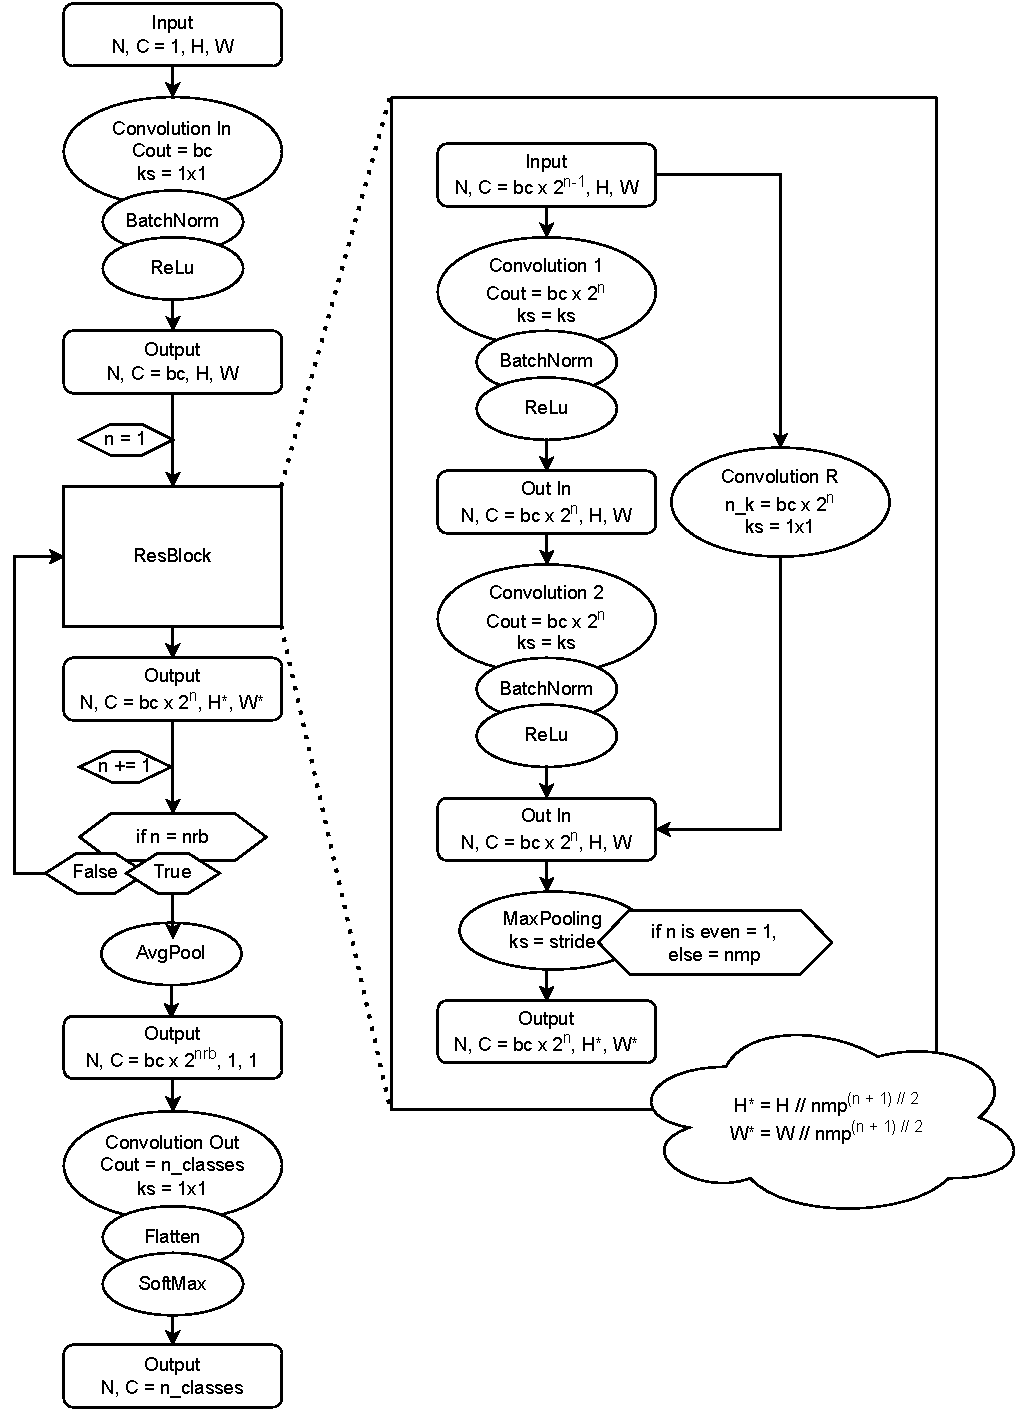
\includegraphics[width=1\textwidth]{figures/model_flow_chart.pdf}
    \caption{
        Flow chart illustrating the models architecture. N: elements in batch, C: channels, H: height, W: width,
        Cout: output channels, ks: kernel size, bc: base channels, nrb: number of residual blocks,
        n\_classes: number of classes, nmp: parameter for max pooling
        }
    \label{fig:model_flow_chart}
\end{figure}


\subsection{Data Processing}
A custom Dataloader was implemented, to handle the data processing on the fly
and provide the trainer with then data samples matching the chosen indices.
To implement the dataloader, the PyTorch Dataset and DataLoader classes where used.
For the data processing, the torchaudio and numpy libraries where used.
There is two steps to the data processing: Sampling and Transformation.

\subsubsection{Sampeling}
The audio files are of different lengths and the model can only handle inputs of a fixed size.
Since the smallest files are of a length of around 1 second and the longest file is around
160 seconds, a compromise had to be made. To only sample the files to a length of 1 second
would mean very little information being available for the model to learn from. On the other
hand if the files are sampled for a length of more than a second, the short files would need
to be padded with zeros meaning the file starts with a basically empty part. This could lead
to the model learning from the length of the empty part and not the actual audio signal.
To avoid this, the audio files where sampled to a random length between 1 and 10 seconds and
then padded with zeros to the fixed length of 10 seconds. To implement this, a custom method
was implemented as shown in Listing \ref{lst:sampeling}.

\begin{lstlisting}[
    language=Python, 
    caption={Python code for the sampeling of the filies}, 
    label={lst:sampeling}]
import numpy as np
import torch

def get_random_part_padded(self, waveform: Tensor, samplerate: int) -> Tensor:

    min_len_in_samples = int(self.min_len_in_seconds * samplerate)
    max_len_in_samples = int(self.max_len_in_seconds * samplerate)

    if self.min_len_in_seconds == -1:
        sample_start_index = -max_len_in_samples
        sample_end_index = None

    else:
        part_length = np.random.randint(min_len_in_samples, max_len_in_samples + 1)
        sample_length = waveform.shape[1]
        part_length = min(part_length, sample_length)
        sample_start_index = np.random.randint(0, sample_length - part_length + 1)
        sample_end_index = sample_start_index + part_length

    waveform_part = waveform[:, sample_start_index:sample_end_index]
    actual_part_length = waveform_part.shape[1]
    pad_length = max_len_in_samples - actual_part_length
    waveform_pad = torch.nn.functional.pad(waveform_part, pad=(pad_length, 0, 0, 0))

    return waveform_pad
\end{lstlisting}


\subsubsection{Transformation}
The model is actually one, usually used for image classification and therefore expects
two dimensional input while an audio file has only one dimension. To transform the samples into
into a format, that the model can handle, a short time Fourier transformation  (STFT) was applied.
The Fourier transformation is a mathematical operation that transforms a function of time
into a function of frequency. An other way to describe this is, that a series of spectrograms
for short time slices of the audio signal are created and aligned in a 2D array - basically
a visualization of the audio signal and therefore something a image classification model can handle.
In addition a second version was implemented, where the STFT where transformed additionally.
The two versions are visualized for a random sample with no padding in Figure \ref{fig:transformations}.
The frequency bins were transformed into mel bins, which are a more human like representation
of the frequency content of the audio signal. This transformation is called a mel-spectrogram
and is commonly used in the field of ecoacoustics \autocite[7]{stowellComputationalBioacousticsDeep2022}.
Both versions of the transformation where transformed into decibels and normalized before 
being passed into the model.

\begin{figure}[h]
    \centering
    \captionsetup{width=.7\linewidth}
    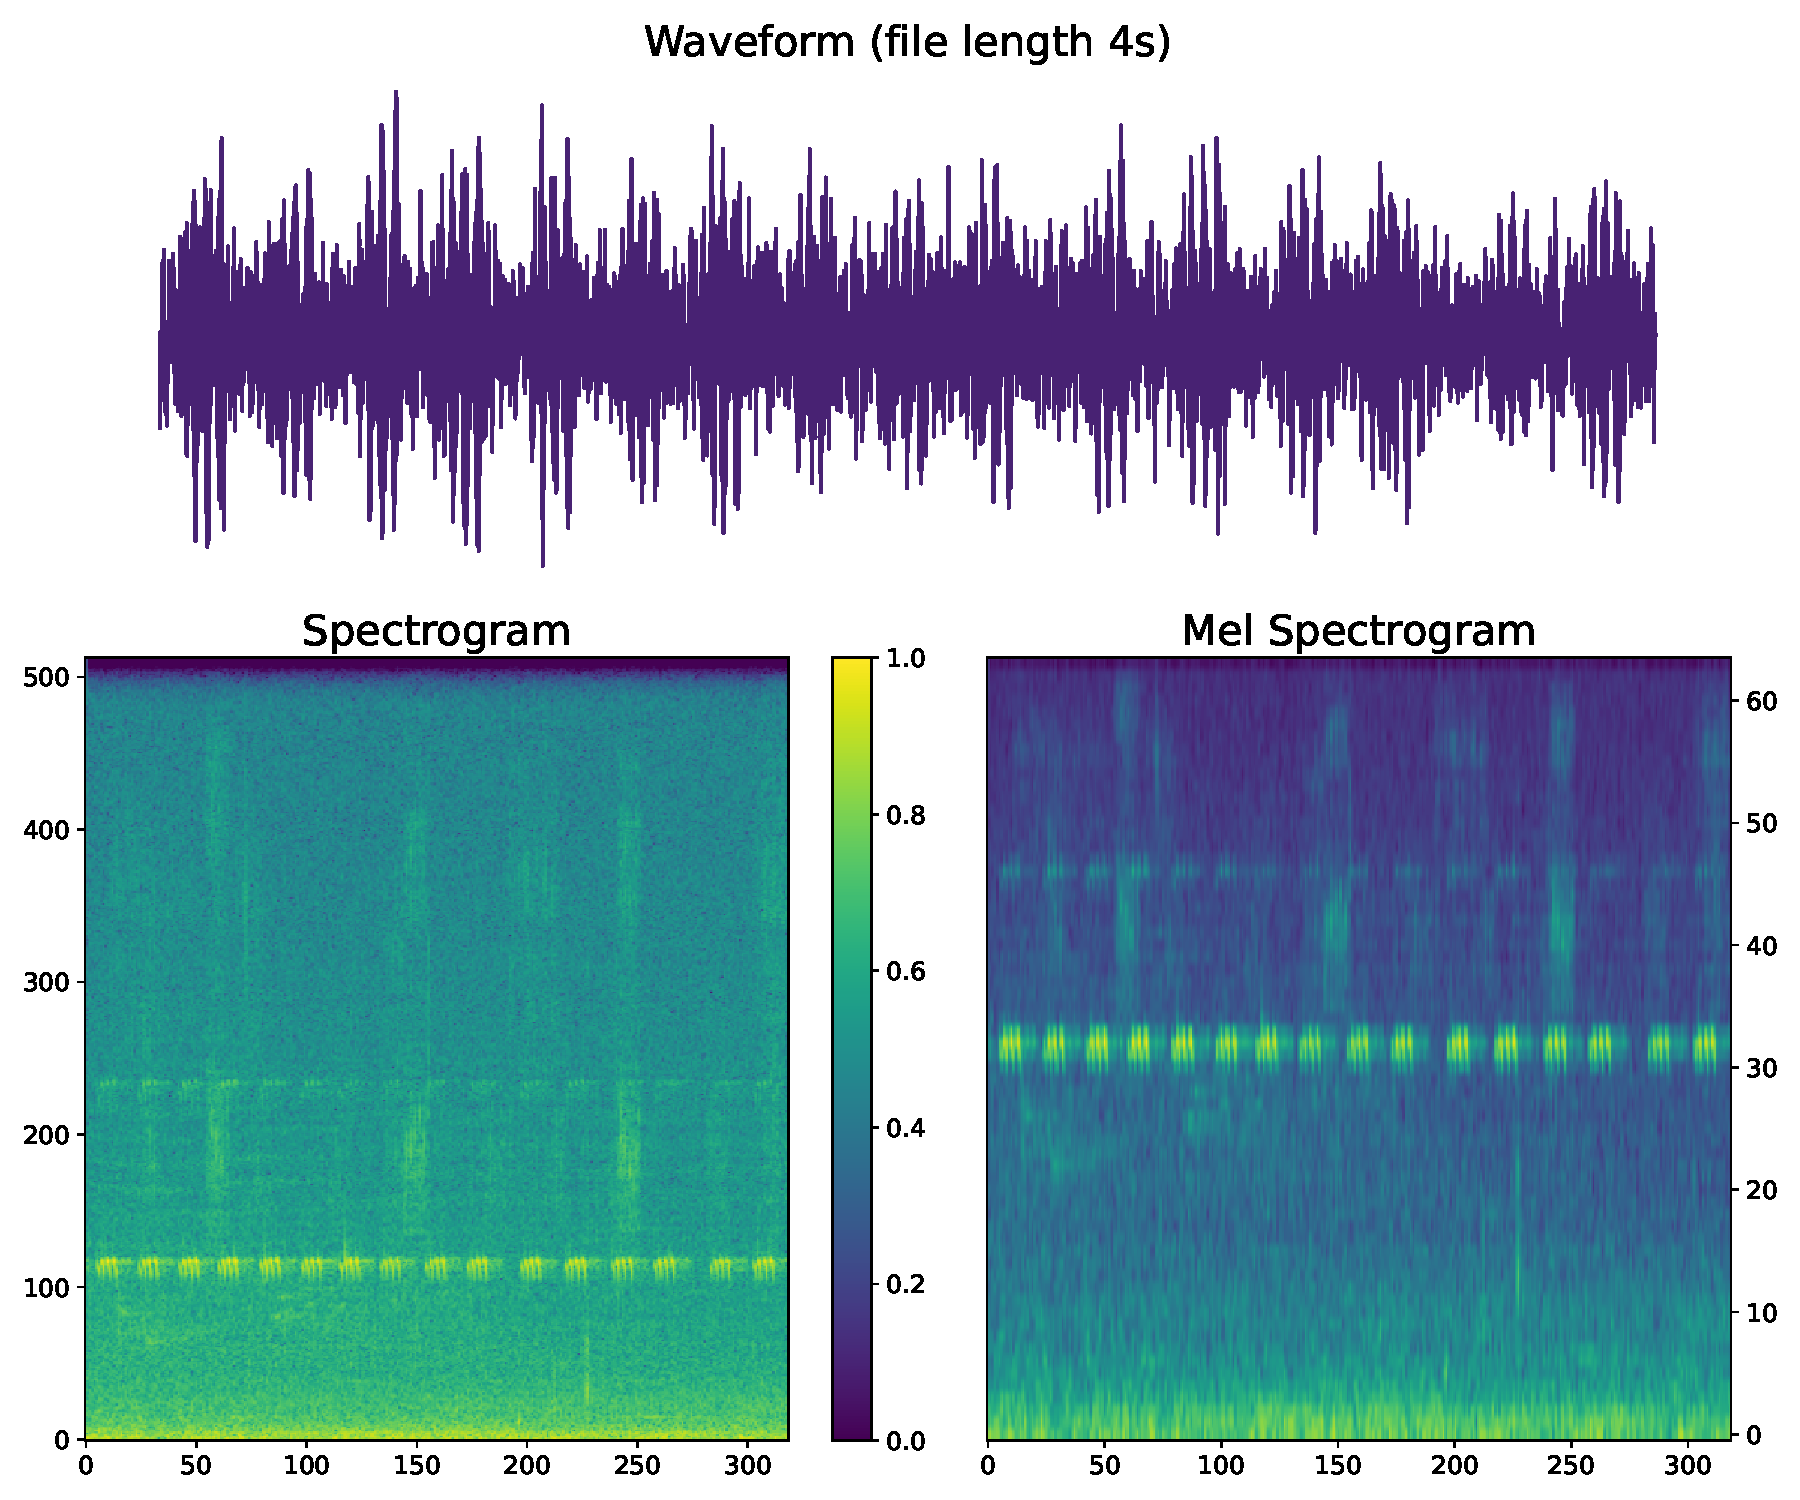
\includegraphics[width=0.85\textwidth]{figures/compare_spectrogram.pdf}
    \caption{Visualization of the two transformations of the audio signal.}
    \label{fig:transformations}
\end{figure}

To implement the two varieties of the transformation, the library torch and torchaudio where used.
A custom transformation method was implemented, that can be used as a layer in the model as shown in 
Listing \ref{lst:transformation}. Some of the parameters of the transformation where made configurable
and others dependant on them where calculated. In the hyperparameter tuning phase, the only parameter
that was tuned was the number of mel bins, which was set to either 64 to try the mel-spectrogram or -1
to use the standard spectrogram.

    \begin{lstlisting}[
        language=Python, 
        caption={Python code for the transformation of the audio signal}, 
        label={lst:transformation}]
    import torch
    import torchaudio

    class NormalizeSpectrogram(torch.nn.Module):
        def forward(self, tensor):
        return (tensor - tensor.min()) / (tensor.max() - tensor.min())

    normalize_transform = NormalizeSpectrogram()

    if n_mels == -1:
        spectrogram = torchaudio.transforms.Spectrogram(
            n_fft=n_fft, 
            hop_length=int(n_fft/2), 
            win_length=n_fft)
    else:
        spectrogram = torchaudio.transforms.MelSpectrogram(
            n_fft=n_fft,
            hop_length=int(n_fft/2),
            win_length=n_fft,
            n_mels=n_mels,
            f_max=self.sample_rate / 2)

    db_transform = torchaudio.transforms.AmplitudeToDB(top_db=top_db)

    self.transform = torch.nn.Sequential(
        spectrogram, 
        db_transform, 
        normalize_transform)
    \end{lstlisting}


\subsection{Fitting the Model}

The training was completely handled by the PyTorch Lightning framework. The logging was done
with the TensorBoard logger and with an additional custom logger to get easier access to the
data afterwards. The hyperparameter grid search was implemented with a custom Python script.

\subsubsection{Training}

The training was done on a single GPU. The model was trained for a maximum of 2000 epochs
with a early stopping callback, that stopped the training if the validation loss did not improve
for patience = 100 epochs. The model was trined with a batch size of 10. The optimizer used was the AdamW
optimizer of the PyTorch library with a weight decay of 0. The loss function used was the
CrossEntropyLoss function of the PyTorch library with default parameters and class weights
according to available data per class. Different learning rates where tried during the hyperparameter
tuning referred to in Section \ref{hyperparameter_tuning}. Only the best model was saved and used for
the evaluation of the model. In order to simplify the evaluation, on completion of the training
the whole dataset was predicted and saved to a csv file in the log folder.

\subsubsection{Hyperparameter Tuning}
\label{hyperparameter_tuning}

For the hyperparameter tuning, a select number of hyperparameters where chosen to be tuned.
Considerations like the experience of some early tests, the computational resources available
and the time frame of the project where taken into account. The hyperparameters that where
chosen for the grid search are shown in Table \ref{tab:hyperparameters}. For the grid search,
models for all possible combinations of the hyperparameters - 
in this case \( 2 \times 3 \times 2 \times 3 = 36 \) where trained. To implement the grid search a short Python
script was written to create the system commands to start the training with the different
hyperparameter combinations.
\begin{table}[h]
    \centering
    \caption{Hyperparameters and values used for the grid search.}
    \label{tab:hyperparameters}
    \begin{tabular}{|l|l|l|l|}
    \hline
    \textbf{Hyperparameter} & \textbf{Description}                  & \textbf{Variations}   & \textbf{Values} \\ \hline
    n\_mels                 & transformation (-1 for regular STFT)  & 2                     & 64, -1 \\ \hline
    n\_res\_blocks          & number of res blocks                  & 3                     & 2, 3, 4 \\ \hline
    learning\_rate          & step size during optimization         & 2                     & 0.001, 0.0001 \\ \hline
    kernel\_size            & dimension of the filter               & 3                     & 3, 5, 7 \\ \hline
    \end{tabular}

\end{table}

